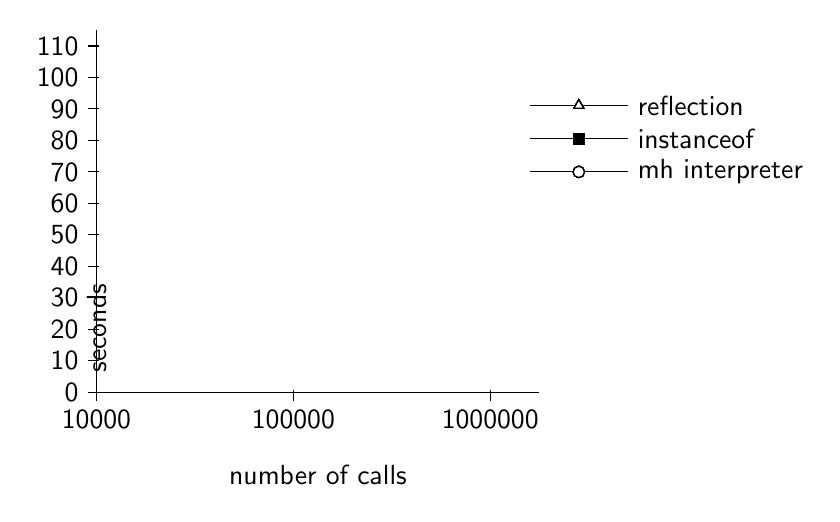
\begin{tikzpicture}[y=.04cm, x=2.5cm,font=\sffamily]
  %axis
  \draw (0,0) -- coordinate (x axis mid) (2.25,0);
      \draw (0,0) -- coordinate (y axis mid) (0,115);
      %ticks
      \draw (0,1pt) -- (0,-3pt) node[anchor=north] {10000};
      \draw (1,1pt) -- (1,-3pt) node[anchor=north] {100000};
      \draw (2,1pt) -- (2,-3pt) node[anchor=north] {1000000};
      \foreach \y in {0,10,...,110}
        \draw (1pt,\y) -- (-3pt,\y) node[anchor=east] {\y}; 
  %labels      
  \node[below=0.8cm] at (x axis mid) {number of calls};
  \node[rotate=90, left=0.8cm] at (y axis mid) {seconds};

  %plots
  \draw plot[mark=*, mark options={fill=white}] 
    file {mcs_indy.data};
  \draw plot[mark=square*]
    file {mcs_instanceof.data};
  \draw plot[mark=triangle*, mark options={fill=white}]
    file {mcs_reflection.data};  

  %legend
  \begin{scope}[shift={(2.2,70)}] 
    \draw (0,0) -- 
      plot[mark=*, mark options={fill=white}] (0.25,0) -- (0.5,0) node[right]{mh interpreter};
    \draw[yshift=\baselineskip] (0,0) -- 
      plot[mark=square*] (0.25,0) -- (0.5,0) node[right]{instanceof};
    \draw[yshift=2\baselineskip] (0,0) -- 
      plot[mark=triangle*, mark options={fill=white}] (0.25,0) -- (0.5,0) node[right]{reflection};
  \end{scope}
\end{tikzpicture}